\documentclass[11pt]{article}

\usepackage{enumitem}
\usepackage{amsmath}
\usepackage{amssymb}
\usepackage{bm}
\usepackage{listings}
\usepackage{color}
\usepackage{tikz}
\usepackage[T1]{fontenc}
\usepackage{courier}
\usepackage{circuitikz}
\usetikzlibrary{calc}
\usepackage{changepage}
\usepackage{multirow}
\usepackage[margin=1.0in]{geometry}
\usepackage[open]{bookmark}

\lstset{xleftmargin=-1cm,
	xrightmargin=\parindent,
	numbersep=5pt} 

\definecolor{dkgreen}{rgb}{0,0.6,0}
\definecolor{gray}{rgb}{0.5,0.5,0.5}
\definecolor{mauve}{rgb}{0.58,0,0.82}

\lstset{
	frame=tb,
	language=Verilog,
	aboveskip=3mm,
	belowskip=3mm,
	showstringspaces=false,
	columns=flexible,
	basicstyle={\small\ttfamily},
	numbers=none,
	numberstyle=\tiny\color{gray},
	keywordstyle=\color{blue},
	commentstyle=\color{dkgreen},
	stringstyle=\color{mauve},
	breaklines=true,
	breakatwhitespace=true,
	tabsize=3,
	xleftmargin=0pt,
}

\title{CS152B Lab 1}

\begin{document}
	
\title{\vspace{-0.5in} Com Sci 152B Digital Design \\
	Lab 2: State Machine Design }
\date{}
\maketitle
\vspace{-0.75in}
\begin{center}
	\begin{tabular}{cc}
		Michael Hale & 004-620-459 \\ 
		Matthew Nuesca & 904-440-067 \\ 
		Shilin Patel & 904-569-866 \\ 
		Bingxin Zhu & 704-845-969
	\end{tabular}
\end{center}

\section{Overview}
In this lab we implemented a simulated traffic intersection on the FPGA development board. The design revolved around a state machine which would transition based on input signals from the street sensor and the walk button. 

\section{Design Requirements}
The design implements the traffic and walk signals for a four way intersection with no protected turns. The traffic light pattern repeats the following cycle:
\begin{enumerate}
	\item Main St begins with a 12-second green light.
	\begin{enumerate}
		\item If the traffic sensor is high after 6 seconds, move to the next step after only 3 additional seconds.
	\end{enumerate}
	\item Main St has a 2-second yellow light.
	\item If the walk button has been pressed and not serviced, illuminate the walk signal for 3 seconds.
	\item Side St has a 6-second green light.
	\begin{enumerate}
		\item If the traffic sensor is high at the end of 6 seconds, remain green for an additional 3 seconds.
	\end{enumerate}
	\item Side St has a 2-second yellow light.
\end{enumerate} 

\section{Implementation Details}
\subsection{State Machine}
Our state machine breaks up each green light into two parts each. The first represents the minimum amount of time a green light can remain on and the second represents the extra time. 

In general, we initialize a counter upon state transition with a value determined by the destination state. For each clock edge (speaking of a 1 Hz clock), we decrement the counter until it reaches zero, at which point we transition to the next state. The first green state for Main St is unique in that it must check the status of the traffic signal without changing states. 

Below is an illustrated state diagram where each state has an explicit counter init value. We describe the variables in the picture as follows:
\begin{itemize}
	\item \texttt{cnt}: Counter variable.
	\item \texttt{sig}: Side St traffic signal.
	\item \texttt{chk}: Checked value of traffic signal after Main St has been on for 6 seconds.
	\item \texttt{walk}: Independently updated walk register. 
\end{itemize}

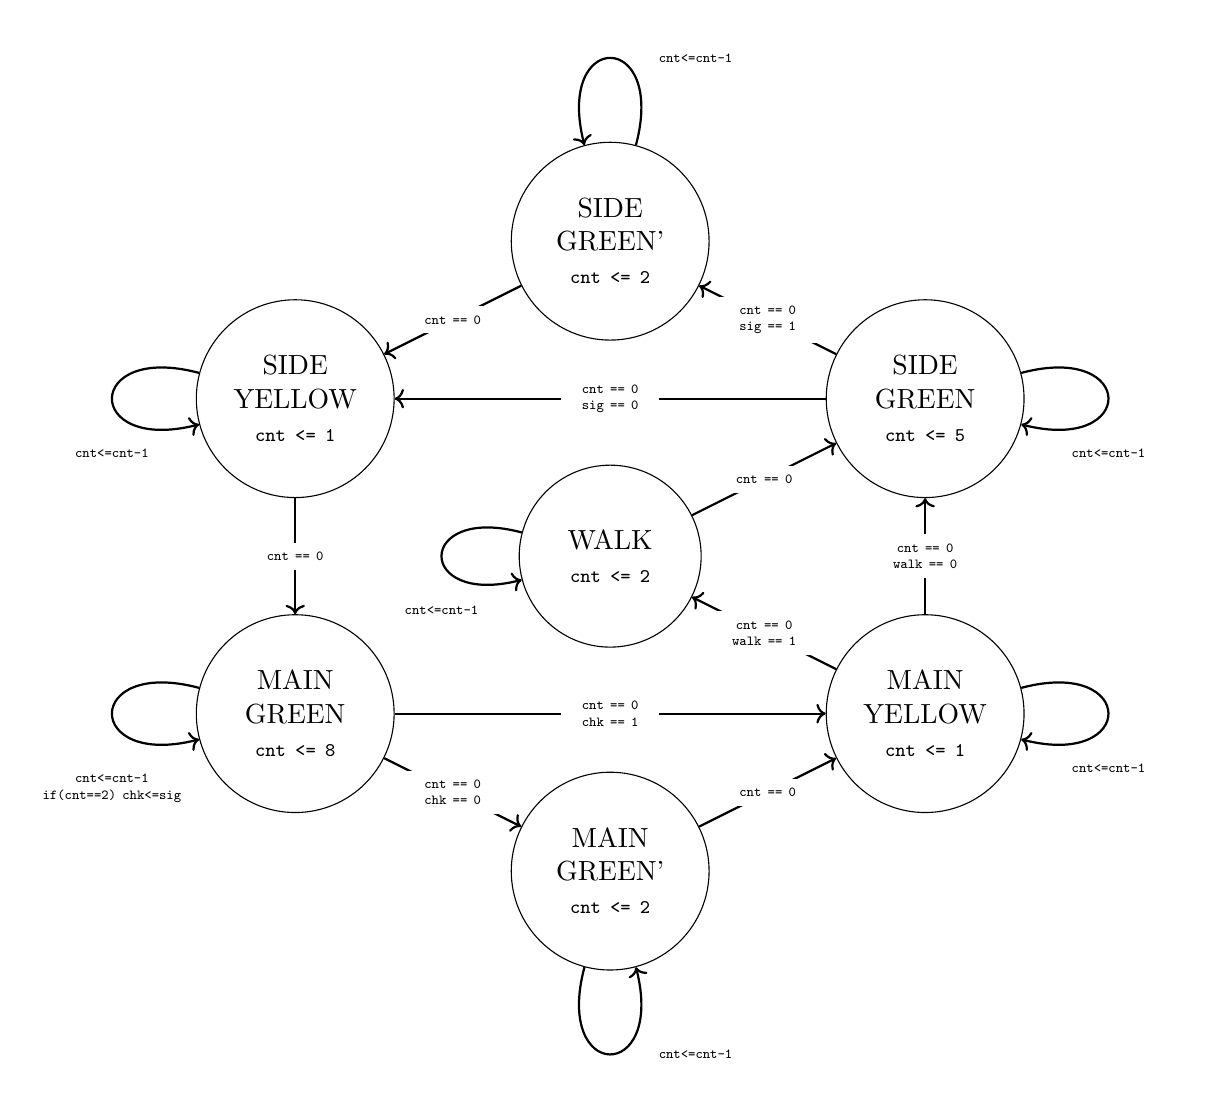
\begin{tikzpicture}
\path (0,0) node[circle,align=center,text width=0.75in,draw](main-green) {MAIN GREEN \scriptsize\texttt{cnt <= 8}};
\path (4,-2) node[circle,align=center,text width=0.75in,draw](main-green-extra) {MAIN GREEN' \scriptsize\texttt{cnt <= 2}};
\path (8,0) node[circle,align=center,text width=0.75in,draw](main-yellow) {MAIN YELLOW \scriptsize\texttt{cnt <= 1}};
\path (0,4) node[circle,align=center,text width=0.75in,draw](side-yellow) {SIDE YELLOW \scriptsize\texttt{cnt <= 1}};
\path (4,6) node[circle,align=center,text width=0.75in,draw](side-green-extra) {SIDE GREEN' \scriptsize\texttt{cnt <= 2}};
\path (8,4) node[circle,align=center,text width=0.75in,draw](side-green) {SIDE GREEN \scriptsize\texttt{cnt <= 5}};
\path (4,2) node[circle,align=center,text width=0.75in,draw](walk) {WALK \scriptsize\texttt{cnt <= 2}};

\draw[->, thick] (main-green) -- (main-green-extra) node[fill=white, font=\tiny, midway, text width=0.4in, text centered] {\texttt{cnt == 0 chk == 0}};
\draw[->, thick] (main-green) -- (main-yellow) node[fill=white, font=\tiny, midway, text width=0.4in, text centered] {\texttt{cnt == 0 chk == 1}};
\draw[->, thick] (main-green-extra) -- (main-yellow) node[fill=white, font=\tiny, midway, text width=0.4in, text centered] {\texttt{cnt == 0}};
\draw[->, thick] (main-yellow) -- (side-green) node[fill=white, font=\tiny, midway, text width=0.45in, text centered] {\texttt{cnt == 0 walk == 0}};
\draw[->, thick] (side-green) -- (side-green-extra) node[fill=white, font=\tiny, midway, text width=0.4in, text centered] {\texttt{cnt == 0 sig == 1}};
\draw[->, thick] (side-green) -- (side-yellow) node[fill=white, font=\tiny, midway, text width=0.4in, text centered] {\texttt{cnt == 0 sig == 0}};
\draw[->, thick] (side-green-extra) -- (side-yellow) node[fill=white, font=\tiny, midway, text width=0.4in, text centered] {\texttt{cnt == 0}};
\draw[->, thick] (side-yellow) -- (main-green) node[fill=white, font=\tiny, midway, text width=0.4in, text centered] {\texttt{cnt == 0}};
\draw[->, thick] (main-yellow) -- (walk) node[fill=white, font=\tiny, midway, text width=0.45in, text centered] {\texttt{cnt == 0 walk == 1}};
\draw[->, thick] (walk) -- (side-green) node[fill=white, font=\tiny, midway, text width=0.4in, text centered] {\texttt{cnt == 0}};

\draw[->, thick] (main-green) to [out=165, in=195, looseness=6] node[font=\tiny, below=0.25in, text width=0.75in, text centered] {\texttt{cnt<=cnt-1 if(cnt==2) chk<=sig}} (main-green);

\draw[->, thick] (main-yellow) to [out=15, in=-15, looseness=6] node[font=\tiny, below=0.2in, text width=0.75in, text centered] {\texttt{cnt<=cnt-1}} (main-yellow);

\draw[->, thick] (main-green-extra) to [out=255, in=285, looseness=6] node[font=\tiny, right, text width=0.75in, text centered] {\texttt{cnt<=cnt-1}} (main-green-extra);

\draw[->, thick] (side-green) to [out=15, in=-15, looseness=6] node[font=\tiny, below=0.2in, text width=0.75in, text centered] {\texttt{cnt<=cnt-1}} (side-green);

\draw[->, thick] (side-green-extra) to [out=75, in=105, looseness=6] node[font=\tiny, right, text width=0.75in, text centered] {\texttt{cnt<=cnt-1}} (side-green-extra);

\draw[->, thick] (side-yellow) to [out=165, in=195, looseness=6] node[font=\tiny, below=0.2in, text width=0.75in, text centered] {\texttt{cnt<=cnt-1}} (side-yellow);

\draw[->, thick] (walk) to [out=165, in=195, looseness=6] node[font=\tiny, below=0.2in, text width=0.75in, text centered] {\texttt{cnt<=cnt-1}} (walk);

\end{tikzpicture}

The Verilog code to implement the state machine was rather trivial, except for when the machine is in the MAIN GREEN state. Here we must check the traffic signal when the counter reaches 2--six seconds after the counter was initialized to 8.

\begin{lstlisting}
case(state)
	MAIN_GREEN: begin
		if(second_cnt == 0) begin
			/* Cut the green light short */
			if (sensor_check == 1) begin 
				state <= MAIN_YELLOW;
				second_cnt <= 1;
			/* Continue for 3 more seconds */
			end else begin 
				state <= MAIN_GREEN_EXTRA;
				second_cnt <= 2;
			end
		/* Check the sensor after 6 seconds */
		end else if (second_cnt == 2) begin
			sensor_check <= side_sensor;
		end 
	end
	...
\end{lstlisting}

Since these states don't correspond to individual traffic light bulbs, we must implement that logic independently:

\begin{lstlisting}
/* Main St lights (G,Y,R) */
assign led[0] = state == MAIN_GREEN || state == MAIN_GREEN_EXTRA;
assign led[1] = state == MAIN_YELLOW;
assign led[2] = state != MAIN_GREEN && state != MAIN_GREEN_EXTRA 
	&& state != MAIN_YELLOW;
/* Side St lights (G,Y,R) */
assign led[3] = state == SIDE_GREEN || state == SIDE_GREEN_EXTRA;
assign led[4] = state == SIDE_YELLOW;
assign led[5] = state != SIDE_GREEN && state != SIDE_GREEN_EXTRA 
	&& state != SIDE_YELLOW;
/* Walk signal */
assign led[6] = state == WALK;
\end{lstlisting}

\subsection{Clock Divider}
To implement our traffic light in hardware, we needed to generate two clock signals. A 1 Hz clock to run our state machine and a 32 Hz clock for the button debouncer. We implemented our clock divider in verilog using two counter registers. The first generated clock signal inverts after 50 million clock edges and the second inverts after 1,562,500 clock edges. 

\subsection{Button Debouncer}
We wanted to ensure our walk button did not generate any noisy signals by filtering the raw button input with a debouncing circuit. Essentially we only check the raw input on a slow clock edge, generating a sampled version of the input signal. We implement this in the following Verilog code:

\begin{lstlisting}
module debouncer(
	input button,
	input clk,
	output reg deb
);

always @(posedge clk) begin
	deb <= button;
end

endmodule
\end{lstlisting}

\section{Testbech}

\section{Challenges \& Solutions}

\end{document}